\documentclass[11pt]{article}
\input{/Users/markwang/.preamble}
\begin{document}


\section*{Chapter 6 Multiple Regression I}

\subsection*{
    \href[page=248]{../apply_linear_model_kutner.pdf}{6.1} Multiple Regression Models}

\begin{enumerate}
    \item \textbf{Need for Several Predictor Variables} A single predictor is often inadequate since often multiple variables affect the response variable in important and distinctive ways, this is especially true for observational experiments where predictor variables are not controlled. Even in controlled experiments, we often want to investigate a number of predictor variables simultaneously 
    \item \textbf{First-Order Model with Two Predictor Variables} A first order model is linear in predictor variables. A first-order model with 2 predictor variable is given by 
    \[
        Y_i = \beta_0 + \beta_1 X_{i1} + \beta_2 X_{i2} + \epsilon_i
    \]
    with regression function as
    \[
        \E\{ Y \} = \beta_0 + \beta_1 X_1 + \beta_2 X_2 
    \]
    A regression function in multiple regression is called a \textbf{regression surface} or a \textbf{response surface}. Parameter $\beta_1$ indicates the change in mean response $\E\{Y\}$ per unit increase in $X_1$ when $X_2$ is held constant. Hence, effect of $X_1$ on mean does not depend on levels of $X_2$, and vice versa, the predictor variables are said to have \textbf{additive effects}or \textbf{not to interact}. Paramters $\beta_1$ and $\beta_2$ are called \textbf{partial regression coefficients} since they reflect on partial effect of one predictor variable when other predictor variables is included in the model and is held constant. 
    \[
        \frac{\partial \E\{Y\}}{\partial X_1} = \beta_1 
        \quad \quad 
        \frac{\partial \E\{Y\}}{\partial X_2} = \beta_2
    \]
    \item \textbf{First-order model with More Than Two Predictor Variables} Consider $p-1$ predictor variables $X_1, \cdots, X_{p-1}$. A first-order model with $p-1$ predictor variables is given by
    \[
        Y_i = \beta_0 + \beta_1 X_{i1} + \beta_2 X_{i2} + \cdots + \beta_{p-1}X_{i, p-1} + \epsilon_i
    \]
    or equivalently
    \[
        Y_i = \beta_0 + \sum_{k=1}^{p-1} \beta_k X_{ik} + \epsilon_i
    \]
    Given $\E\{ \epsilon_i \} = 0$, the regression function is given by
    \[
        \E\{Y\} = \beta_0 + \beta_1 X_1 + \cdots + \beta_{p-1}X_{p-1}
    \]
    which represents a \textbf{hyperplane}. Parameter $\beta_k$ indicates change in the mean response $\E\{Y\}$ with a unit increase in predictor variable $X_k$, when all other predictor variables in the regression model are held constant
    \item \textbf{General Linear Regression Model} A general linear model, with normal error terms, is given by 
    \[
        Y_i = \beta_0 + \beta_1 X_{i1} + \beta_2 X_{i2} + \cdots + \beta_{p-1}X_{i, p-1} + \epsilon_i 
    \]
    where 
    \begin{enumerate}
        \item $\beta_0, \beta_1, \cdots, \beta_{p-1}$ are parameters 
        \item $X_{i1}, \cdots, X_{i, p-1}$ are known constants 
        \item $\epsilon_i$ are independent $\norm(0, \sigma^2)$
    \end{enumerate}
    with response function given by 
    \[
        \E\{Y\} = \beta_0 + \beta_1 X_1 + \beta_2 X_2 + \cdots + \beta_{p-1}X_{p-1} \tag{$\E\{\epsilon_i\}=0$}
    \]
    The general linear model usage cases
    \begin{enumerate}
        \item \textbf{$p-1$ Predictor Variables} as seen with first-order model with $p-1$ predictor variables, which has no interactione ffects
        \item \textbf{Qualitative Predictor Variables} Indicator variables as $X_i$s. As an example of 1 quantitative predictor $X_{i1}$ and 1 indicator predictor variable $X_{i2}$
        \[
            \E\{Y\} = \beta_0 + \beta_1 X_1 + \beta_2 X_2 
        \]
        We have 2 response function 
        \[
            \E\{Y\} = \beta_0 + \beta_1 X_1 
            \quad \quad \quad 
            \E\{Y\} = (\beta_0 + \beta_2) + \beta_1 X_1
        \]
        which represents parallel straight lines with different intercepts. Generally we represents qualitative variable with $c$ classes by means of $c-1$ indicator variables 
    \end{enumerate}
    \item \textbf{Polynomial Regression} is a special case of generalized linear model contaiing higher-order terms of predictor variable, making the response function curlinear. For example 
    \[
        Y_i = \beta_0 + \beta_1 X_i + \beta_2 X_i^2 + \epsilon_i
    \]
    where $X_{i1} = X_i$ and $X_{i2} = X_i^2$
    \item \textbf{Transformed Variables}
    \item \textbf{Interaction Effects} When effects of predictor variables on response variable are not additive, the effect of one predictor variable depends on levels of other predictor variables. A \textbf{nonadditive regressfion model with 2 predictors $X_1$ and $X_2$} is given by 
    \[
        Y_i = \beta_0 + \beta_1 X_{i1} + \beta_2 X_{i2} + \beta_3 X_{i1}X_{i2} + \epsilon_i
    \]
    which is a special case of generalized linear model whereby $X_{i3} = X_{i1}X_{i2}$
    \item \textbf{Combination of above cases} For example, model that is curlinear with interaction terms.
    \item \textbf{Meaning of linear in General Linear Regression Model} Note GLM does is not restricted to linear response surfaces. \textbf{Linear Model} refers to the fact that model is linear in the parameters; it does not refer to the shape of the response surface. 
    \[
        Y_i  =\beta_0 exp(\beta_1 X_i) + \epsilon
    \]
    is a nonlinear regression model 
\end{enumerate}




\subsection*{
    \href[page=256]{../apply_linear_model_kutner.pdf}{6.2-6.3} General Linear Regression Model in Matrix Terms} 


\begin{enumerate}
    \item \textbf{GLR Model in Matrix} \\
    Given 
    \[
        \underset{n\times 1}{\matr{Y}} = 
        \begin{bmatrix}
            Y_1 \\ Y_2 \\ \vdots \\ Y_n \\ 
        \end{bmatrix}
        \quad 
        \underset{n\times p}{\matr{X}} = 
        \begin{bmatrix}
            1 & X_{11} & X_{12} & \cdots & X_{1, p-1} \\ 
            1 & X_{21} & X_{22} & \cdots & X_{2, p-1} \\ 
            \vdots & \vdots & \vdots & & \vdots \\
            1 & X_{n1} & X_{n2} & \cdots & X_{n, p-1} \\ 
        \end{bmatrix}
        \quad 
        \underset{p\times 1}{\beta} = 
        \begin{bmatrix}
            \beta_0 \\ \beta_1 \\ \vdots \\ \beta_{p-1} \\ 
        \end{bmatrix}
        \quad 
        \underset{n\times 1}{\epsilon} = 
        \begin{bmatrix}
            \epsilon_1 \\ \epsilon_2 \\ \vdots \\ \epsilon_n
        \end{bmatrix}
    \]
    The model is given by 
    \[
        \matr{Y = X\boldsymbol{\beta} + \boldsymbol{\epsilon}}
    \]
    where
    \[
        \underset{n\times n}{\matr{\sigma^2\{\boldsymbol{\epsilon}\}}} = 
        \begin{bmatrix}
            \sigma^2 & 0 & \cdots & 0 \\
            0 & \sigma^2 & \cdots & 0 \\
            \vdots & \vdots & & \vdots \\
            0 & 0 & \cdots & \sigma^2 \\ 
        \end{bmatrix}
        = \sigma^2 \matr{I}
    \]
    So the expectation of response given by 
    \[
        \E\{Y\} =  \matr{X\boldsymbol{\beta}} \quad \quad \matr{\sigma^2\{Y\}} = \sigma^2 \matr{I}
    \]
    \item \textbf{Estimation of Regression Coefficients} \\
    Idea is to minimize least squared 
    \[
        Q = \sum_i^n (Y_i - \beta_0 - \beta_1 X_{i1} - \cdots - \beta_{p-1}X_{i, p-1})^2
    \]
    minimize $Q$ to get normal equation 
    \[
        \matr{X'X\boldsymbol{\hat{\beta}} = X'Y}
    \]
    yielding least squared estimator 
    \[
        \boldsymbol{\hat{\beta}} = \matr{(X'X)^{-1}X'Y}
    \]
    \item \textbf{Fitted Values and Residuals} \\
    \begin{align*}
        \matr{\hat{Y}} &= \matr{X\boldsymbol{\hat{\beta}}} \\ 
        \matr{\hat{e}} &= \matr{(I-H)Y} \tag{where $\matr{H} = X(X'X)^{-1}X'$}  \\
        \sigma^2\{\matr{\hat{e}}\} &= \sigma^2\matr{(I-H)} \\ 
        s^2\{\matr{\hat{e}}\} &= MSE(\matr{I-H}) \\ 
    \end{align*}
    \item \textbf{Sum of Squares and Mean Squares} \\
    Same as before 
    \begin{align*}
        SST &= \matr{Y'}\left[ \matr{I} - (\frac{1}{n})\matr{J} \right]\matr{Y}\\
        RSS &= \matr{Y'(1-H)Y}\\ 
        SSReg &= \matr{Y'}\left[ \matr{H} - (\frac{1}{n})\matr{J} \right]\matr{Y}\\
    \end{align*}
    with 
    \begin{enumerate}
        \item SST has $n-1$ degrees of freedom 
        \item RSS has $n-p$ degrees of freedom 
        \item SSReg has $p-1$ degrees of freedom
    \end{enumerate}
    So the mean square is given by
    \begin{align*}
        MSE = \frac{RSS}{n-p}
        MSReg = \frac{SSReg}{p-1}
    \end{align*}
    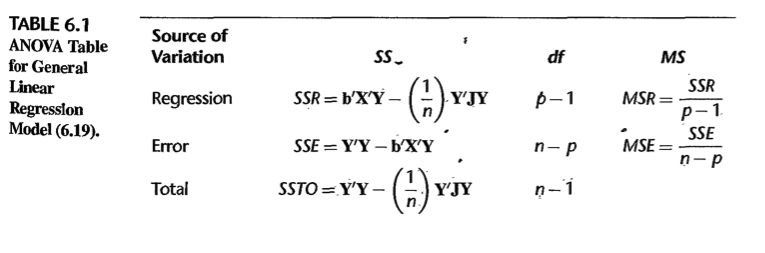
\includegraphics[width=\textwidth]{anova_table_for_GLR.png}
    \item \textbf{F-test for Regression Relation} tests for if there is a regression relation between the response variable $Y$ and the set of $X$ variable $X_1, \cdots, X_{p-1}$
    \[
        \begin{cases}
            \textsc{H}_0: \beta_1 = \beta_2 = \cdots = \beta_{p-1} = 0 \\
            \textsc{H}_{\alpha}: \text{ not all } \beta_{k} \text{ equal zero } k = 1, \cdots, p-1
        \end{cases}
    \]
    With test statistic 
    \[
        F&* = \frac{MSReg}{MSE}
    \]
\end{enumerate}



\end{document}
